\lecture{2}{vendredi 07 février 2020}
\vspace{-1.2cm}

\section{Introduction à la Traduction Automatique (TA)}

\epigraph{(…) the attempt to automate all, or part of the process\\ of translating from one human language to another.}{\textit{Arnold, 1993}}

Définition de Traduction Automatique: Automatisation du processus de traduction d'une $Phrase_{source} \rightarrow Phrase_{cible}$.
Il s'agit d'un domaine en constante évolution. Il envisage l'exercice de traduction comme s'il s'agissait d'un processus de décodage. \\

\noindent Il existe 3 types de traduction automatique:

\begin{enumerate}
    \item \textbf{Assimilation} Rompre la barrière des langues. Comprendre à minima le contenu d'un texte.
    On parle souvent de "gisting". Il y a de nombreuses applications: communication interne, blogs, journaux,
    sites web, documentation, littérature, etc. Il existe peu d'évaluation quantitative de ce genre de traduction.
    De toute façon, comment évaluer une telle traduction? Son but n'est pas d'être optimale, mais juste de couvrir
    au minimum la compréhension du texte source. Autre problème: de nombreux services de traduction online stockent
    les textes source, il y a donc un risque de problèmes de protection des données.
    \item \textbf{Communication} TA pour la communication orale (interprétation). Deux technologies centrales: la synthèse vocale et la TA.
    \item \textbf{Dissémination} TA du traducteur. Son but est de publier un texte dans une autre langue.
    La qualité doit être égale à la TH (traduction humaine), et il y a deux conditions pour que ce soit le cas
    \begin{enumerate}
        \item \textbf{Domaine limité} On essaye d'avoir une TEAHQ (Traduction Entièrement Automatique et de Haute Qualité) / FAHQT (Fully Automatic High Quality Translation).
        Ceci est impossible si on essaye de traduire dans un scope de langage énorme.
        Donc on essaye de focaliser les efforts sur un sous-langage (e.g. un traducteur spécialisé dans le domaine de la météo).
        \item \textbf{Intervention humaine} Un humain (traducteur ou réviseur) intervient dans le processus de traduction,
        de deux façons possibles: pré-édition (simplification du texte, éviter les phrases longues et les longs groupes nominaux, etc)
        et post-édition (PE). De nouveaux métiers se créent (sujet complexe car on dit également que d'autres métiers se perdent).
    \end{enumerate}
\end{enumerate}

\noindent Dans les prochains chapitres on analysera les trois types de systèmes de traduction automatique:

\begin{enumerate}
    \item \textbf{Systèmes linguistiques} Rule-based machine translation (RBMT) \footnote{\hyperref[sec:RBMT]{Chapitre 3}}
    \item \textbf{Systèmes fondés sur les corpus (data-driven)} \footnote{\hyperref[sec:corpus]{Chapitre 4}}
    \begin{enumerate}
        \item Statistical machine translation (SMT)
        \item Neuronal machine translation (NMT) \\
    \end{enumerate}
\end{enumerate}

\noindent\textbf{Post-édition VS Traduction Humaine}
\begin{enumerate}
    \item Rentable, 20\% à 40\% de gain de productivité selon les études (e.g. Plitt \& Masselot 2010, Green 2013)
    \item Ne conduit pas nécessairement à plus d'erreurs ou des textes de moins bonne qualité
    \item "Posteditese" (e.g. Toral 2019, Kubler 2019). I.e. : la post-édition donne lieu à des textes avec des particularités différentes de ceux issus de la traduction humaine.
\end{enumerate}

\newpage

\noindent\textbf{Nouvelles applications de la TA\\}

\begin{minipage}[t]{0.5\textwidth}
\begin{itemize}
\item Sous-titrage
\item TA d'images
\item TA vers des langues simplifiées \\(e.g. Simple Wikipedia)\\
\end{itemize}
\end{minipage}
\begin{minipage}[t]{0.5\textwidth}
\begin{itemize}
\item TA vers des pictogrammes
\item TA vers la langue des signes
\end{itemize}
\end{minipage}

\noindent\textbf{Problèmes posés par la TA}

\begin{enumerate}
    \item \textbf{Ambigüité}
    \begin{enumerate}
        \item Lexicale (e.g. "fumer \textbf{nuit} à la santé" $\rightarrow$ "to smoke \textbf{night} with health")
        \item Structurale (e.g. "he hammers the metal \textbf{flat}" $\rightarrow$ "il martèle \textbf{l'appartement} en métal")
    \end{enumerate}
    \item \textbf{Divergences}
    \begin{enumerate}
        \item Lexicales/Décalages (e.g. "I \textbf{know} this word" $\rightarrow$ "je \textbf{sais} ce mot")
        \item Structurales (e.g. This is a \textbf{good} man $\rightarrow$ c'est un \textbf{bon} homme)
    \end{enumerate}
    \item \textbf{De nombreuses traductions possibles}
        Comment choisir la meilleure (ou la seule correcte)?
\end{enumerate}

\noindent\textbf{Divergences structurales\\}

\begin{enumerate}
    \item Typologiques
    \begin{enumerate}
        \item Ordre des mots (e.g. SVO en FR, SOV en Japonais et VSO en Arabe)
        \item Pronoms
    \end{enumerate}
    \item Idiosyncratiques (propres à une langue)
    \item Générales à la syntaxe d'une langue
    \item Déclenchées par un mot particulier \\
\end{enumerate}

Du plus facile au plus compliqué à résoudre (Vandooren 1993) \\

\begin{enumerate}
    \item Catégorielle (e.g. nom vers adjectif, "\textbf{university} degree" $\rightarrow$ "diplôme \textbf{universitaire}")
    \item Syntagmatique (e.g. "I’m waiting for the postman to pass" $\rightarrow$ "j’attends le passage du facteur")
    \item Lexicale (e.g. "\textbf{I'm} hungry" $\rightarrow$ "\textbf{J'ai} faim")
    \item De densité lexicale (e.g. "he retired" $\rightarrow$ "il a pris sa retraite")
    \item Thématique (e.g. John \textbf{missed} Mary $\rightarrow$ Marie \textbf{a manqué à} Jean)
    \item Prédicative (e.g. "he hammers the metal flat" $\rightarrow$ "il aplatit le métal avec un marteau")\\
\end{enumerate}

\noindent\textbf{Statistiques des divergences (Dorr 2002)\\}

\begin{enumerate}
    \item Part of Speech (98\%)
    \item Phrase/Light verb (83\%)
    \item Structural (35\%)
    \item Heads swap (8\%)
    \item Arguments swap (6\%)
\end{enumerate}

\newpage

\section{Les systèmes linguistiques (RBMT)}
\label{sec:RBMT}

Les premiers systèmes de TA commerciaux et sur internet (BabelFish, Altavista, etc).
Ils étaient les seuls à être développés jusqu'en 2006 (avant l'apparition de SMT et NMT, voir chapitre suivant).

À l'époque ils étaient les seuls à faire de la TEAHQ (à mettre en perspective, la qualité n'est plus considérée aussi bonne quand on la compare aux résultats actuels).

Beaucoup de différences entre ces systèmes, mais quelques points communs:

\begin{enumerate}
    \item \textbf{Analyse linguistique} pour extraire le sens de la phrase
    ("natural language understanding"). Pipeline linguistique (on passe par différents niveaux: lexical,
        syntaxique, sémantique, pragmatique/extralinguistique)
    \item \textbf{Transfert}
    \item \textbf{Génération} de la langue cible\\
\end{enumerate}

\textbf{En résumé}

\begin{enumerate}
    \item Très ambitieux
    \item Hypothèses (fausses)
    \begin{itemize}
        \item Assume qu'il y a beaucoup de régularités entre les langues
        \item Assume qu'il existe peu d'exceptions (grammaires compactes)
        \item Assume que toutes les règles peuvent être définies par des experts
    \end{itemize}
    \item Problèmes
    \begin{itemize}
        \item Robustesse: les langues ne sont pas si régulières
        \item Chers et lents à développer
        \item Statiques: figés dans le temps, n'apprennent pas via de nouveaux corpus
    \end{itemize}
\end{enumerate}

\subsection{Systèmes directs/minimalistes}

Les plus simples, ils reposent sur des dictionnaires énormes faits humainement. Ne peuvent donner des résultats exploitables que si le sous-langage et le dictionnaire sont bien spécialisés.\\

\textbf{Fonctionnement}

\begin{enumerate}
    \item \textbf{Compréhension minimale (lexicale)}: segmentation en mots et tagging de catégorie grammaticale de chaque mot
    \item \textbf{Traduction}: mot à mot avec un dictionnaire bilingue
    \item \textbf{Génération}: flexions, ordre des mots, élision, etc.\\
\end{enumerate}

\textbf{Problèmes}

\begin{enumerate}
    \item \textbf{Compréhension}: Analyse morphologique et résolution des homographes catégoriels. Le système ne voit pas l’ambiguïté structurale des phrases, il reste au niveau lexical.
    \item \textbf{Traduction}: Tests/actions limités. Un dictionnaire par paire de langues.
    \item \textbf{Génération}: Architecture de type "transformateur". Pas de connaissances grammaticales de la langue cible, comme dans les systèmes indirects.\\
\end{enumerate}

\textbf{Dictionnaire}

La ressource principale des systèmes directs (pas de grammaires).

Il contient toutes les informations nécessaires pour la compréhension et la traduction,
c'est à dire au minimum: le mot/expression source/cible, les informations lexicales monolingues sur le mot/expression source/cible et les informations bilingues.\\

\newpage

\textbf{Informations bilingues}

\begin{enumerate}
    \item Traduction mots/expressions
    \item Tests (transfer conditions)
    \begin{itemize}
        \item Permettent de choisir la bonne traduction s'il y en a plusieurs.
        \item Devraient porter sur tous les niveaux linguistiques (lexical, synt, sem et pragmatique).
        \item e.g. : grow (élever, cultiver ou grandir?)
    \end{itemize}
    \item Actions
\end{enumerate}

\textbf{Types de tests}

\begin{itemize}
    \item Test sur les informations morphologiques (e.g. singulier vs pluriel)
    \item Test sur la syntaxe (rection) (e.g. traduction d'un verbe dépendant de
    l'objet auquel il s'applique)
    \item Test sur le type sémantique (sens) (e.g. traduction d'un verbe dépendant
    du type de sujet, humain ou animal)
    \item Test sur le domaine (e.g. le mot "bug" en informatique ou en biologie)
    \item Test sur les propriétés encyclopédiques (ontologie) (e.g. traductions
    entières de bouts de phrases stockées)\\
\end{itemize}

Dans les systèmes directs, les tests portent uniquement sur le niveau lexical:
nombre, genre, mots dans contexte.

Exemple: SystranNet (2018)

to grow (context: child, etc.) = grandir

to grow (context: chicken, etc.) = élever

to grow (context: corn, salad, etc.) = cultiver \\

\textbf{Actions}

Permettent de traiter les divergences, c'est-à-dire de changer la syntaxe sous
certaines conditions. Exemple: "hungry" en anglais qui devient "avoir faim".

\subsection{Systèmes indirects/maximalistes}

Tandis que les systèmes directs focalisaient le moins possible sur le niveau de
la compréhension (minimalistes), les systèmes indirects eux le font au plus possible.

Ils sont les seuls systèmes linguistiques à faire de la TEAHQ.\\

\textbf{Caractéristiques}

\begin{enumerate}
    \item Ne restent pas au niveau lexical. Font au moins une analyse syntaxique complète, avec une grammaire, et représentent ainsi le sens de la phrase à traduire.
    \item Ne mettent pas en relation directe des mots, mais mettent en correspondance des représentations.
\end{enumerate}

\textbf{Avantages}

\begin{enumerate}
    \item Les représentations rendent explicites plus d'informations qui peuvent être ainsi utilisées pour la traduction.
    \item Facilitent le lien entre les langues.
    \item Représentent l’ambigüité structurale. (e.g. Fumer nuit/v à la santé)
\end{enumerate}

\newpage

\textbf{Fonctionnement}

\begin{enumerate}
    \item Représentation: devrait contenir ce que les traducteurs rendent explicites quand ils traduisent
    \item Deux approches
        \begin{itemize}
            \item Par transfert: peut-on se limiter à une représentation spécifique à chaque langue?
            \item Par interlangue: faut-il définir une représentation indépendante des langues? \\
        \end{itemize}
\end{enumerate}

\textbf{Différences transfert VS interlangue}

\begin{enumerate}
    \item Types de représentation: similaire ou pas pour les langues?
    \item Connaissances contrastives
    \item Type de traduction
    \begin{itemize}
        \item Transfert: littérale, on préserve la syntaxe
        \item Interlangue: par paraphrase, on va vers le sens et on génère avec le sens de la phrase
    \end{itemize}
\end{enumerate}

\vspace{1cm}

\textbf{Triangle de Vauquois}

\resizebox{0.85\textwidth}{!}{
    

\tikzset{every picture/.style={line width=0.75pt}} %set default line width to 0.75pt

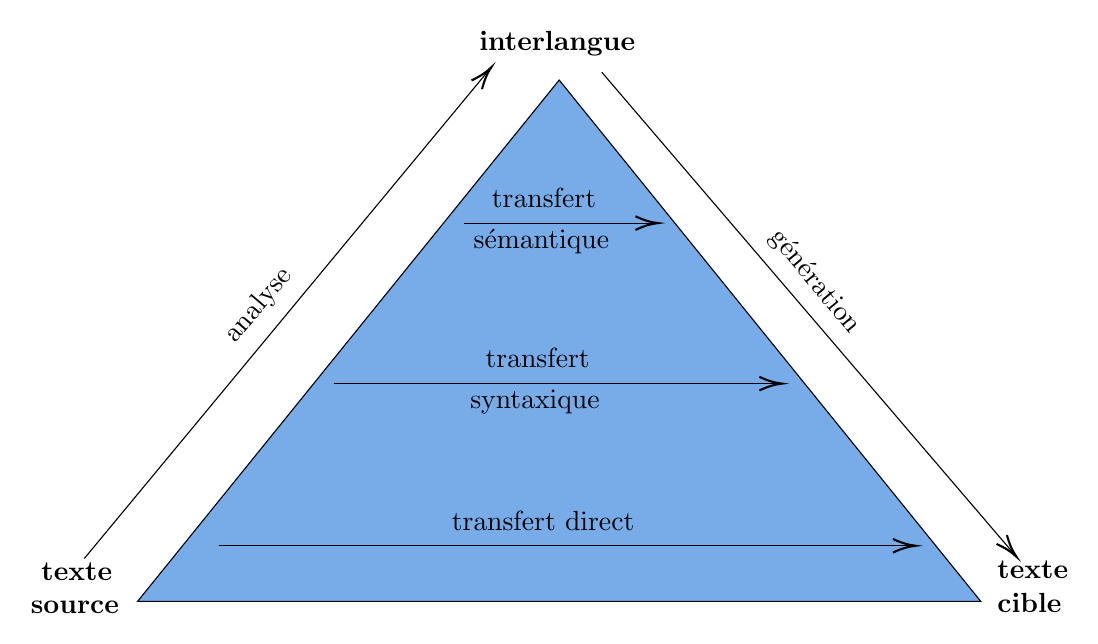
\begin{tikzpicture}[x=0.75pt,y=0.75pt,yscale=-1,xscale=1]
%uncomment if require: \path (0,777); %set diagram left start at 0, and has height of 777

%Shape: Triangle [id:dp37993567465978106]
\draw  [fill={rgb, 255:red, 74; green, 144; blue, 226 }  ,fill opacity=0.75 ] (297.6,38.51) -- (500.73,289.68) -- (94.48,289.68) -- cycle ;
%Straight Lines [id:da3821484196531547]
\draw    (133.92,262.88) -- (467.33,262.88) ;
\draw [shift={(469.33,262.88)}, rotate = 180] [color={rgb, 255:red, 0; green, 0; blue, 0 }  ][line width=0.75]    (10.93,-3.29) .. controls (6.95,-1.4) and (3.31,-0.3) .. (0,0) .. controls (3.31,0.3) and (6.95,1.4) .. (10.93,3.29)   ;
%Straight Lines [id:da35117354484946606]
\draw    (189.05,184.77) -- (403.01,184.77) ;
\draw [shift={(405.01,184.77)}, rotate = 180] [color={rgb, 255:red, 0; green, 0; blue, 0 }  ][line width=0.75]    (10.93,-3.29) .. controls (6.95,-1.4) and (3.31,-0.3) .. (0,0) .. controls (3.31,0.3) and (6.95,1.4) .. (10.93,3.29)   ;
%Straight Lines [id:da19792780780087094]
\draw    (251.85,107.43) -- (343.28,107.43) ;
\draw [shift={(345.28,107.43)}, rotate = 180] [color={rgb, 255:red, 0; green, 0; blue, 0 }  ][line width=0.75]    (10.93,-3.29) .. controls (6.95,-1.4) and (3.31,-0.3) .. (0,0) .. controls (3.31,0.3) and (6.95,1.4) .. (10.93,3.29)   ;
%Straight Lines [id:da14845116336104136]
\draw    (68.83,269.01) -- (263.59,33.92) ;
\draw [shift={(264.87,32.38)}, rotate = 489.64] [color={rgb, 255:red, 0; green, 0; blue, 0 }  ][line width=0.75]    (10.93,-3.29) .. controls (6.95,-1.4) and (3.31,-0.3) .. (0,0) .. controls (3.31,0.3) and (6.95,1.4) .. (10.93,3.29)   ;
%Straight Lines [id:da355143642126483]
\draw    (318.12,34.73) -- (516.63,266.67) ;
\draw [shift={(517.93,268.19)}, rotate = 229.44] [color={rgb, 255:red, 0; green, 0; blue, 0 }  ][line width=0.75]    (10.93,-3.29) .. controls (6.95,-1.4) and (3.31,-0.3) .. (0,0) .. controls (3.31,0.3) and (6.95,1.4) .. (10.93,3.29)   ;

% Text Node
\draw (257.83,13.54) node [anchor=north west][inner sep=0.75pt]   [align=left] {\textbf{{interlangue}}};
% Text Node
\draw (507.5,269.15) node [anchor=north west][inner sep=0.75pt]   [align=left] {\textbf{texte}\\\textbf{cible}};
% Text Node
\draw (41.79,269.92) node [anchor=north west][inner sep=0.75pt]   [align=left] {\textbf{ texte}\\\textbf{source}};
% Text Node
\draw (244.58,244.81) node [anchor=north west][inner sep=0.75pt]   [align=left] {transfert direct};
% Text Node
\draw (260.87,166.7) node [anchor=north west][inner sep=0.75pt]   [align=left] {transfert};
% Text Node
\draw (253.52,186.61) node [anchor=north west][inner sep=0.75pt]   [align=left] {syntaxique};
% Text Node
\draw (263.94,89.35) node [anchor=north west][inner sep=0.75pt]   [align=left] {transfert};
% Text Node
\draw (255.12,109.26) node [anchor=north west][inner sep=0.75pt]   [align=left] {sémantique};
% Text Node
\draw (132.51,159.58) node [anchor=north west][inner sep=0.75pt]  [rotate=-310.5] [align=left] {analyse};
% Text Node
\draw (406.04,106.74) node [anchor=north west][inner sep=0.75pt]  [rotate=-50.3] [align=left] {génération};


\end{tikzpicture}

}

\vspace{1cm}

Axe vertical: profondeur d'analyse, niveau d'analyse syntaxique
    e.g. directs on reste au niveau lexical, transfert au moins syntaxique, interlingue on va jusqu'au niveau sémantique

Axe horizontal: quantité de connaissance contrastive qu'il faut pour passer d'une langue à l'autre \\

\subsubsection{Systèmes par transfert}

\begin{itemize}
    \item Module d'analyse: syntaxique et spécifique à la langue (par définition)
    \item Module de transfert: règles de transfert
    \item Génération: Représentation syntaxique cible $\rightarrow$ texte cible\\
\end{itemize}

\textbf{Types de règles de transfert}

\begin{itemize}
    \item Lexicales: équivalences entre les mots
    \item Structurales: liens entre les éléments structuraux (e.g. verb $\rightarrow$ verbe, subject $\rightarrow$ sujet)
    \item Semi-lexicales: permettent de changer la syntaxe de la phrase via des tests et actions\\
\end{itemize}

\textbf{Avantages}

\begin{itemize}
    \item Séparation des connaissances monolingues et bilingues.
    \item Connaissances de la grammaire cible (grammaire). Moins de fautes dans la langue cible.
    \item Tests valides. (e.g. know + phrase = savoir VS know + GN = connaître)
    \item Les connaissances syntaxiques aident grandement à écrire les actions. (e.g. inverser sujet/objet)
\end{itemize}

\subsubsection{Systèmes par interlangue}

\textbf{Problèmes}

\begin{itemize}
    \item Concepts: définir l'ensemble des concepts et choisir le bon contexte. Ceci oblige à faire des distinctions qui ne sont pas nécessaires pour toutes les paires de langues. E.g. espagnol: différence entre le mot pour poisson vivant et poisson mort.
    \item Granularité de la représentation.\\
\end{itemize}


\textbf{Exemples d'interlangue}

\begin{itemize}
    \item Pour la langue générale: UNL Universal Networking Language (ONU), Nespole!, Esperanto, DLT Distributed Language Translation
    \item Pour des domaines limités: Kantoo, Kant, Tamerlan, Dionysus
    \item Systèmes commerciaux: Atlas II (Fujitsu, Uchida), PIVOT (Nec)\\
\end{itemize}

\textbf{Contexte positif pour l'interlangue}

\begin{itemize}
    \item Sous domaine, si possible technique (terminologie): travail humain énorme
    \item Contexte multilingue: un seul système, au lieu d'un système par chaque paire de langues
    \item Langues très différentes: e.g. Japonais, le transfert ne fonctionne pas vu la différence énorme au niveau de la grammaire
\end{itemize}
